\Opensolutionfile{ans}[ans/ansTN-BTX-101]

\noindent \textbf{PHẦN I. Câu trắc nghiệm nhiều phương án lựa chọn. Thí sinh trả lời từ câu 1 đến câu 12. Mỗi câu hỏi thí sinh chỉ chọn một phương án}
\vspace{0.2cm}

\begin{ex}	\macau{ID: VL12-BTX101-C01}Khi nói về nội năng, khẳng định nào sau đây là đúng?
	\choice
	{Nội năng của A lớn hơn nội năng của B thì nhiệt độ của A cũng lớn hơn nhiệt độ của B}
	{\True Nội năng là một dạng năng lượng}
	{Nội năng là nhiệt lượng}
	{Nội năng của vật chỉ thay đổi trong quá trình truyền nhiệt, không thay đổi trong quá trình thực hiện công}
	\loigiai{
		Nội năng là một dạng năng lượng bên trong của hệ (bằng tổng động năng chuyển động nhiệt và thế năng tương tác của các phân tử cấu tạo nên vật), nội năng phụ thuộc vào cả nhiệt độ và thể tích nên phương án B đúng}
\end{ex}

\begin{ex}	\macau{ID: VL12-BTX101-C02}Một khối chất (có thể là chất rắn kết tinh, hoặc chất lỏng, hoặc chất khí) đang nhận nhiệt lượng nhưng nhiệt độ của nó không thay đổi. Khối chất đó
	\choice
	{\True đang chuyển thể}
	{lại là chất khí}
	{là chất lỏng}
	{là chất rắn}
	\loigiai{
		Khi một khối chất đang tiến hành quá trình chuyển thể (ví dụ: đang nóng chảy hoặc đang sôi), nó liên tục nhận nhiệt lượng từ bên ngoài nhưng nhiệt lượng này chỉ phục vụ phá vỡ các liên kết cấu trúc giữa các hạt chứ không làm gia tăng động năng chuyển động nhiệt, do đó nhiệt độ của hệ được giữ nguyên không đổi}
\end{ex}

\begin{ex}	\macau{ID: VL12-BTX101-C03}Điểm đóng băng và điểm sôi của nước tinh khiết dóng theo thang nhiệt độ Fahrenheit tương ứng lần lượt là
	\choice
	{$0^\circ\text{F}$ và $100^\circ\text{F}$}
	{$100^\circ\text{F}$ và $200^\circ\text{F}$}
	{$22^\circ\text{F}$ và $202^\circ\text{F}$}
	{\True $32^\circ\text{F}$ và $212^\circ\text{F}$}
	\loigiai{
		Theo quy ước của nhiệt giai Fahrenheit, điểm đóng băng của nước tinh khiết ở áp suất tiêu chuẩn được chọn làm mốc $32^\circ\text{F}$ và điểm sôi của nước được chọn làm mốc vạch $212^\circ\text{F}$}
\end{ex}

\begin{ex}	\macau{ID: VL12-BTX101-C04}Trong hệ thống đo lường SI, đơn vị đo tiêu chuẩn của đại lượng nhiệt dung riêng là
	\choice
	{\True $\text{J/(kg.K)}$}
	{$\text{J/(g.K)}$}
	{$\text{cal/(kg}^\circ\text{C)}$}
	{$\text{cal/(g}^\circ\text{C)}$}
	\loigiai{
		Nhiệt dung riêng $c$ được xác định theo hệ thức: $c = \frac{Q}{m \cdot \Delta T}$. Trong hệ SI, nhiệt lượng $Q$ đo bằng Jun ($\text{J}$), khối lượng $m$ đo bằng kilôgam ($\text{kg}$) và nhiệt độ đo bằng Kelvin ($\text{K}$), do đó đơn vị tiêu chuẩn là $\text{J/(kg.K)}$}
\end{ex}

\begin{ex}	\macau{ID: VL12-BTX101-C05}Một chất ở thể rắn như iodine (I-ốt), băng phiến, đá khô ($\text{CO}_2$ ở thể rắn),... có thể chuyển trực tiếp sang ......(1)....... khi nó ......(2)....... Hiện tượng trên gọi là sự thăng hoa. Hãy chọn cụm từ thích hợp điền vào chỗ trống.
	\choice
	{(1) thể hơi; (2) tỏa nhiệt}
	{(1) thể lỏng; (2) nhận nhiệt}
	{\True (1) thể hơi; (2) nhận nhiệt}
	{(1) thể lỏng; (2) tỏa nhiệt}
	\loigiai{
		Sự thăng hoa là quá trình biến đổi trạng thái chuyển pha trực tiếp của một chất từ thể rắn sang thể hơi (thể khí) mà không cần đi qua trạng thái thể lỏng trung gian, đây là quá trình thu nhiệt nên chất cần nhận nhiệt. Do đó (1) thể hơi; (2) nhận nhiệt}
\end{ex}

\begin{ex}	\macau{ID: VL12-BTX101-C06}Tính độ biến thiên nội năng của một hệ vật chất khi vật thực hiện hấp thụ một nhiệt lượng có độ lớn bằng $25\text{ kJ}$ từ môi trường và đồng thời thực hiện sinh ra một công cơ học có độ lớn bằng $15\text{ kJ}$.
	\choice
	{$-10\text{ kJ}$}
	{\True $10\text{ kJ}$}
	{$-40\text{ kJ}$}
	{$40\text{ kJ}$}
	\loigiai{
		Theo quy ước dấu của Nguyên lí I nhiệt động lực học:
		- Vật hấp thụ nhiệt lượng $\Rightarrow Q = +25\text{ kJ}$.
		- Vật thực hiện công (sinh công) ra bên ngoài $\Rightarrow A = -15\text{ kJ}$.
		Độ biến thiên nội năng của hệ vật:
		$$\Delta U = Q + A = 25 + (-15) = +10\text{ kJ}$$
		Nội năng tăng một lượng bằng $10\text{ kJ}$}
\end{ex}

\begin{ex}	\macau{ID: VL12-BTX101-C07}Nhiệt kế nào sau đây hoạt động dựa trên nguyên lí hiện tượng dãn nở vì nhiệt tự nhiên của chất lỏng mao dẫn?
	\choice
	{Nhiệt kế điện tử}
	{Nhiệt kế hồng ngoại}
	{\True Nhiệt kế thủy ngân}
	{Nhiệt kế kim loại}
	\loigiai{
		Nhiệt kế thủy ngân (và các dạng nhiệt kế rượu chất lỏng) hoạt động dựa vào nguyên lí đo sự thay đổi thể tích, dãn nở dài vì nhiệt của cột chất lỏng chứa bên trong bầu đo mao dẫn}
\end{ex}

\begin{ex}	\macau{ID: VL12-BTX101-C08}Thiết bị nào sau đây \textbf{không} được sử dụng trong bộ dụng cụ thí nghiệm dùng để xác định nhiệt dung riêng của nước?
	\begin{center}
		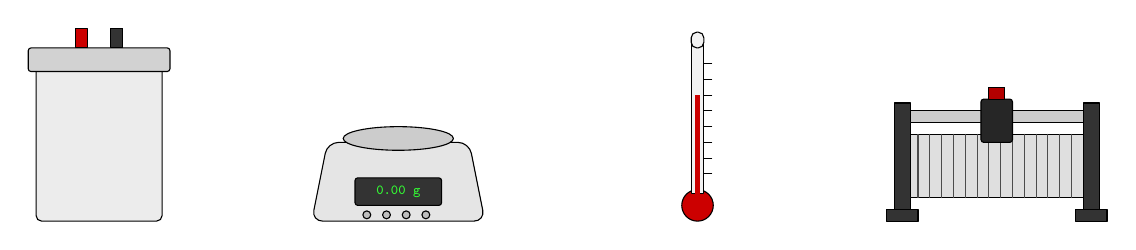
\begin{tikzpicture}[>=stealth, font=\footnotesize, line cap=round, line join=round]
			% A. Nhiet luong ke
			\begin{scope}[xshift=0cm]
				\draw[fill=gray!15, rounded corners=2pt] (-0.8,0) rectangle (0.8,2.0);
				\draw[fill=gray!35, rounded corners=1pt] (-0.9,1.9) rectangle (0.9,2.2);
				\draw[fill=red!80!black] (-0.3,2.2) rectangle (-0.15,2.45);
				\draw[fill=black!80] (0.15,2.2) rectangle (0.3,2.45);
			\end{scope}

			% B. Can dien tu
			\begin{scope}[xshift=3.8cm]
				\draw[fill=gray!20, rounded corners=4pt] (-1.1,0) -- (1.1,0) -- (0.9,1.0) -- (-0.9,1.0) -- cycle;
				\draw[fill=gray!40] (0,1.05) ellipse (0.7cm and 0.15cm);
				\draw[fill=black!80, rounded corners=1pt] (-0.55,0.2) rectangle (0.55,0.55);
				\node[text=green!80!white, font=\tiny\ttfamily] at (0,0.37) {0.00 g};
				\foreach \x in {-0.4, -0.15, 0.1, 0.35} {
					\draw[fill=gray!50] (\x, 0.08) circle (0.05);
				}
			\end{scope}

			% C. Nhiet ke
			\begin{scope}[xshift=7.6cm]
				\draw[fill=red!80!black] (0,0.2) circle (0.2);
				\draw[fill=gray!10] (-0.08,0.35) rectangle (0.08,2.3);
				\draw[rounded corners=2pt, fill=gray!10] (-0.08,2.2) rectangle (0.08,2.4);
				\draw[fill=red!80!black, draw=none] (-0.03,0.2) rectangle (0.03,1.6);
				\foreach \y in {0.6,0.8,1.0,1.2,1.4,1.6,1.8,2.0} {
					\draw[line width=0.3pt] (0.08,\y) -- (0.18,\y);
				}
			\end{scope}

			% D. Bien tro con chay
			\begin{scope}[xshift=11.4cm]
				\draw[fill=black!80] (-1.3,0) -- (-1.1,0) -- (-1.1,1.5) -- (-1.3,1.5) -- cycle;
				\draw[fill=black!80] (1.1,0) -- (1.3,0) -- (1.3,1.5) -- (1.1,1.5) -- cycle;
				\draw[fill=black!80] (-1.4,0) rectangle (-1.0,0.15);
				\draw[fill=black!80] (1.0,0) rectangle (1.4,0.15);
				\draw[fill=gray!25] (-1.1,0.3) rectangle (1.1,1.1);
				\foreach \x in {-1.0,-0.85,-0.7,-0.55,-0.4,-0.25,-0.1,0.05,0.2,0.35,0.5,0.65,0.8,0.95} {
					\draw[line width=0.4pt, color=black!70] (\x,0.3) -- (\x,1.1);
				}
				\draw[fill=gray!40] (-1.1,1.25) rectangle (1.1,1.4);
				\draw[fill=black!85, rounded corners=1pt] (-0.2,1.0) rectangle (0.2,1.55);
				\draw[fill=red!70!black] (-0.1,1.55) rectangle (0.1,1.7);
			\end{scope}
		\end{tikzpicture}
	\end{center}
	\choice
	{Nhiệt lượng kế}
	{Cân điện tử}
	{Nhiệt kế}
	{\True Biến trở}
	\loigiai{
		Trong bài thực hành đo nhiệt dung riêng của nước lỏng, ta cần cân điện tử để đo khối lượng nước $m$, nhiệt kế đo độ biến thiên nhiệt độ $\Delta T$, nhiệt lượng kế ngăn thất thoát năng lượng. Biến trở không cần thiết dùng trong phép đo cơ bản này}
\end{ex}

\begin{ex}	\macau{ID: VL12-BTX101-C09}Điều nào sau đây \textbf{sai} khi phát biểu định tính về đặc điểm cấu trúc mô hình của chất ở thể rắn?
	\choice
	{Sự sắp xếp của các phân tử có tính trật tự tuần hoàn chặt chẽ}
	{Các phân tử chỉ dao động nhiệt quanh một vị trí cân bằng cố định xác định}
	{\True Các phân tử chỉ dao động quanh vị trí cân bằng và bản thân vị trí cân bằng này liên tục dời chỗ chuyển động hỗn loạn}
	{Khoảng cách không gian giữa các phân tử rất gần nhau (cỡ kích thước phân tử)}
	\loigiai{
		Ở thể rắn, các lực liên kết phân tử là vô cùng mạnh mẽ giữ cho các hạt chỉ có thể dao động nhiệt quanh một vị trí cân bằng cố định xác định, không thể dời chỗ tự do. Do đó nhận định C phát biểu vị trí cân bằng chuyển động hỗn loạn là sai}
\end{ex}

\begin{ex}	\macau{ID: VL12-BTX101-C10}Một bình nhiệt lượng kế chứa nước ở nhiệt độ ban đầu $25^\circ\text{C}$ được đun nóng ổn định bằng một dây điện trở nhiệt cấp dòng đều. Đồ thị nào sau đây biểu diễn đúng sự phụ thuộc của nhiệt độ theo thời gian đun của nước lỏng trước khi đạt đến ngưỡng sôi?
	\begin{center}
		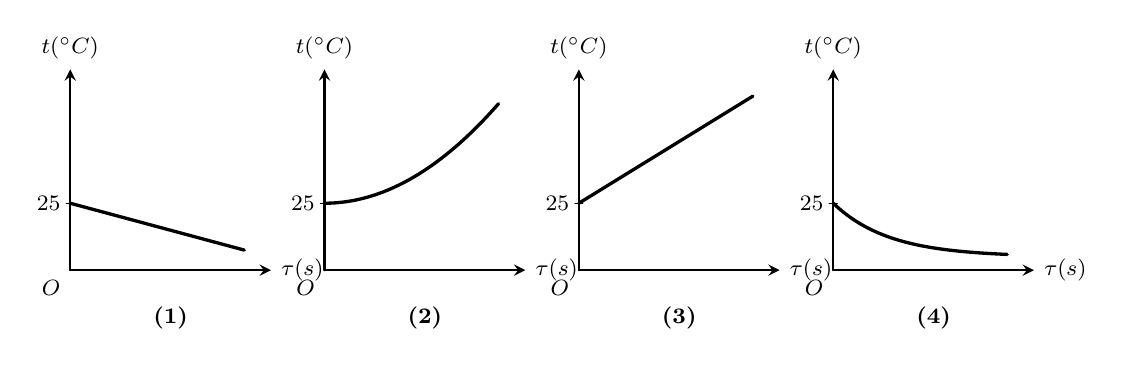
\begin{tikzpicture}[>=stealth, font=\footnotesize, scale=0.85, line cap=round, line join=round]
			\foreach \i/\labelname in {1/(1), 2/(2), 3/(3), 4/(4)} {
				\begin{scope}[xshift={(\i-1)*3.8cm}]
					% Trục tọa độ
					\draw[->, thick] (0, 0) -- (3.0, 0) node[right] {$\tau(\text{s})$};
					\draw[->, thick] (0, 0) -- (0, 3.0) node[above] {$t(^\circ\text{C})$};
					% Gốc tọa độ và vạch chia 25
					\node[below left] at (0, 0) {$O$};
					\node[left] at (0, 1) {$25$};
					\draw (-0.06,1) -- (0.06,1);
					% Nhãn đồ thị phía dưới
					\node[below] at (1.5, -0.4) {\textbf{\labelname}};
					% Vẽ các đường biểu diễn tương ứng
					\ifnum\i=1
					\draw[very thick] (0, 1) -- (2.6, 0.3);
					\fi
					\ifnum\i=2
					\draw[very thick, samples=50] plot[domain=0:2.6] (\x, {1 + 0.22*\x*\x});
					\fi
					\ifnum\i=3
					\draw[very thick] (0, 1) -- (2.6, 2.6);
					\fi
					\ifnum\i=4
					\draw[very thick, samples=50] plot[domain=0:2.6] (\x, {0.2 + 0.8*exp(-1.2*\x)});
					\fi
				\end{scope}
			}
		\end{tikzpicture}
	\end{center}
	
	\choice
	{Đồ thị (2) (Đường cong hướng lên)}
	{\True Đồ thị (3) (Đường thẳng dốc hướng lên đi từ vạch số 25)}
	{Đồ thị (4) (Đường cong hướng xuống)}
	{Đồ thị (1) (Đường thẳng dốc hướng xuống)}
	\loigiai{
		Công suất tỏa nhiệt cung cấp ổn định $P = \text{const} \Rightarrow Q = P \cdot \tau$. Mặt khác, nhiệt lượng thu vào nâng nhiệt chất lỏng tăng đều: $Q = m \cdot c \cdot (t - t_0)$. \\
		Đồng nhất hệ thức: $P \cdot \tau = m \cdot c \cdot (t - 25) \Rightarrow t = \left(\frac{P}{m \cdot c}\right)\tau + 25$. \\
		Hàm số phụ thuộc của nhiệt độ $t$ theo biến số thời gian $\tau$ có cấu trúc là một hàm bậc nhất dạng tuyến tính dốc hướng lên, xuất phát từ vạch thềm nhiệt độ đầu $25^\circ\text{C}$, ứng với Đồ thị (3)}
\end{ex}

\begin{ex}	\macau{ID: VL12-BTX101-C11}Hệ thức quy ước dấu nào dưới đây phù hợp với quá trình một khối khí lý tưởng chứa trong một xi-lanh kín đang giãn nở sinh công đẩy tấm pít-tông dời chỗ ra ngoài mà không nhận nhiệt?
	\choice
	{$\Delta U=Q; Q>0$}
	{$\Delta U=A; A>0$}
	{$\Delta U=Q; Q<0$}
	{\True $\Delta U=A; A<0$}
	\loigiai{
		Khối khí giãn nở đẩy pít-tông tức là hệ thực hiện công sinh công lực ra ngoại cảnh, theo quy ước dấu Nguyên lí I công đại số mang giá trị âm: $A < 0$. Do quá trình không trao đổi nhiệt ($Q=0$), hệ thức phù hợp là $\Delta U = A$ với $A < 0$}
\end{ex}

\begin{ex}	\macau{ID: VL12-BTX101-C12}Điều nào sau đây phát biểu hoàn toàn đúng khi đề cập đến đặc điểm cấu trúc mô hình của chất ở thể khí?
	\choice
	{\True Các phân tử chuyển động hoàn toàn hỗn loạn không ngừng về mọi hướng}
	{Các phân tử chỉ dao động nhiệt quanh một vị trí cân bằng cố định}
	{Sự sắp xếp không gian của các phân tử có tính trật tự tuần hoàn cao}
	{Khoảng cách trung bình giữa các phân tử là rất gần nhau}
	\loigiai{
		Ở thể khí, các lực liên kết tương tác giữa các phân tử là vô cùng yếu ớt, khoảng cách giữa chúng rất lớn nên các phân tử tự do tịnh tiến và chuyển động hỗn loạn không ngừng về mọi hướng, chiếm toàn bộ dung tích bình chứa}
\end{ex}

\Closesolutionfile{ans}

%%%%%%%%%%%%%%%%%%%%%%%%%%%%%%%%%%%%%%%%%%%%%%%%%%%%%%%%%%%%%%%%%%%%%%%%%
% PHẦN II: CÂU TRẮC NGHIỆM ĐÚNG SAI
%%%%%%%%%%%%%%%%%%%%%%%%%%%%%%%%%%%%%%%%%%%%%%%%%%%%%%%%%%%%%%%%%%%%%%%%%
\noindent \textbf{PHẦN II. Câu hỏi trắc nghiệm đúng sai. Thí sinh trả lời từ câu 1 đến câu 2. Trong mỗi ý a), b), c), d) ở mỗi câu, thí sinh chọn đúng hoặc sai}
\Opensolutionfile{ans}[ans/ansTF-BTX-101]

\begin{ex}	\macau{ID: VL12-BTX101-C13}Dùng lực cọ xát mạnh liên tục một miếng kim loại đồng xu lên bề mặt sàn nhà tấm gỗ thì ta ghi nhận thấy miếng kim loại nóng dần lên.
	\choiceTF[t]
	{Giá trị nội năng bên trong của miếng kim loại bị suy giảm dần đi trong tiến trình cọ xát}
	{\True Tại bề mặt tiếp xúc hình học giữa miếng kim loại và sàn nhà xuất hiện lực ma sát trượt sinh công cơ học}
	{Hành động cọ xát cơ học trên thực chất là ta đã làm thay đổi nội năng của miếng kim loại bằng phương thức truyền nhiệt thuần túy}
	{\True Khi tiến hành cọ xát cơ học với cường độ mạnh và trong một khoảng thời gian đủ dài, nhiệt năng tích lũy có thể kích thích tạo ra ngọn lửa}
	\loigiai{
		\begin{itemchoice}
			\itemch Miếng kim loại nóng lên chứng tỏ nhiệt độ tăng, dẫn đến động năng chuyển động nhiệt phân tử tăng, kéo theo nội năng của hệ tăng lên, không phải giảm.
			\itemch Lực ma sát xuất hiện cản trở chuyển động trượt sinh công cơ học cản phá chuyển hóa cơ năng thành nội năng của vật.
			\itemch Việc thực hiện chà xát cơ học sinh lực dời chỗ là phương thức biến đổi nội năng bằng con đường \textbf{thực hiện công}, không phải phương thức truyền nhiệt.
			\itemch Công của lực ma sát chuyển hóa liên tục thành nhiệt năng tích tụ, nếu thời gian đủ dài nhiệt độ đạt tới điểm bắt cháy của vật liệu gỗ sàn có thể phát hỏa tạo ra ngọn lửa.
		\end{itemchoice}
	}
\end{ex}

\begin{ex}	\macau{ID: VL12-BTX101-C14}Một học sinh tiến hành thiết lập thí nghiệm đun nóng để làm nóng chảy và hóa hơi hoàn toàn khối lượng $m = 0,02\text{ kg}$ nước đá đang ở điểm nóng chảy $0^\circ\text{C}$ chuyển trọn vẹn thành hơi nước bão hòa ở điểm sôi $100^\circ\text{C}$. Cho biết các hằng số kĩ thuật: hằng số ẩn nhiệt nóng chảy riêng của nước đá là $\lambda = 3,34 \cdot 10^5\text{ J/kg}$; hằng số nhiệt dung riêng của nước lỏng bằng $c = 4200\text{ J/(kg.K)}$; hằng số ẩn nhiệt hóa hơi riêng của nước ở điểm sôi bằng $L = 2,26 \cdot 10^6\text{ J/kg}$ và bỏ qua hoàn toàn các hao phí nhiệt lượng thất thoát ra môi trường ngoài.
	\choiceTF[t]
	{Nhiệt lượng cần thiết cung cấp để làm nóng chảy tan rã hoàn toàn $0,020\text{ kg}$ nước đá tại nhiệt độ nóng chảy có trị số bằng $6860\text{ J}$}
	{\True Nhiệt lượng cần thiết cung cấp để nâng nhiệt độ của khối $0,020\text{ kg}$ nước lỏng sau khi tan từ mức $0^\circ\text{C}$ đạt tiến đến điểm sôi $100^\circ\text{C}$ bằng đúng $8400\text{ J}$}
	{Nhiệt lượng cần thiết tiêu hao cung cấp độc quyền để làm hoá hơi hoàn toàn $0,020\text{ kg}$ nước lỏng đang sôi ở $100^\circ\text{C}$ bằng $42500\text{ J}$}
	{\True Tổng nhiệt lượng toàn phần cần cung cấp cho cả tiến trình chuyển pha vĩ mô từ nước đá $0^\circ\text{C}$ thành hơi nước ở $100^\circ\text{C}$ đạt giá trị bằng $60280\text{ J}$}
	\loigiai{
		\begin{itemchoice}
			\itemch Nhiệt lượng cần thiết cung cấp phục vụ riêng cho quá trình nóng chảy hoàn toàn băng đá:
			$$Q_1 = \lambda \cdot m = 3,34 \cdot 10^5 \cdot 0,02 = 6680\text{ J} \neq 6860\text{ J}$$
			\itemch Nhiệt lượng cấp nâng nhiệt khối nước lỏng ấm lên từ $0^\circ\text{C} \rightarrow 100^\circ\text{C}$:
			$$Q_2 = m \cdot c \cdot \Delta t = 0,02 \cdot 4200 \cdot (100 - 0) = 8400\text{ J}$$
			\itemch Nhiệt lượng cung cấp phục vụ quá trình hóa hơi cưỡng bức bão hòa hoàn toàn lượng nước lỏng:
			$$Q_3 = L \cdot m = 2,26 \cdot 10^6 \cdot 0,02 = 45200\text{ J} \neq 42500\text{ J}$$
			\itemch Tổng nhiệt lượng toàn phần cần thiết tiêu hao cung cấp cho toàn bộ tiến trình biến đổi chuyển pha:
			$$\Sigma Q = Q_1 + Q_2 + Q_3 = 6680 + 8400 + 45200 = 60280\text{ J}$$
		\end{itemchoice}
	}
\end{ex}

\Closesolutionfile{ans}

%%%%%%%%%%%%%%%%%%%%%%%%%%%%%%%%%%%%%%%%%%%%%%%%%%%%%%%%%%%%%%%%%%%%%%%%%
% PHẦN III: CÂU TRẮC NGHIỆM TRẢ LỜI NGẮN
%%%%%%%%%%%%%%%%%%%%%%%%%%%%%%%%%%%%%%%%%%%%%%%%%%%%%%%%%%%%%%%%%%%%%%%%%
\noindent \textbf{PHẦN III. Câu trắc nghiệm trả lời ngắn. Thí sinh trả lời từ câu 1 đến câu 4}
\Opensolutionfile{ans}[ans/ansSA-BTX-101]

\begin{ex}	\macau{ID: VL12-BTX101-C15}Trong một bài thí nghiệm động học, người ta cho thả rơi tự do một mảnh khối vật liệu thép từ độ cao vị trí ban đầu rất lớn bằng $5,00 \cdot 10^3\text{ m}$. Khi khối vật rơi tiến sát sát chạm vào mặt đất, thiết bị ghi nhận tốc độ tức thời của nó đạt ngưỡng $300\text{ m/s}$. Cho biết hằng số nhiệt dung riêng của vật liệu thép bằng $460\text{ J/(kg.K)}$ và lấy gia tốc trọng trường mốc $g = 9,81\text{ m/s}^2$. Hỏi mảnh thép đã bị nóng ấm gia tăng thêm một lượng nhiệt độ bằng bao nhiêu độ khi chạm đất? Biết toàn bộ phần công cơ học của lực cản không khí sinh ra chỉ phục vụ đốt nóng nội năng mảnh thép. (Kết quả lấy làm tròn đến một chữ số sau dấu phẩy thập phân).

	\par\shortans[oly]{87,2}
	\loigiai{
		\begin{itemize}
			\item Định luật bảo toàn và chuyển hóa năng lượng toàn phần chỉ ra: Cơ năng ban đầu tại đỉnh cao chuyển hóa thành động năng chạm đất cộng với phần công cản của không khí sinh ra chuyển thành nhiệt năng làm nóng vật: $W_1 = W_2 + A_{\text{cản}} \Rightarrow mgh = \frac{1}{2}mv^2 + Q_{\text{làm nóng}}$.
			\item Triệt tiêu khối lượng m ở hai vế phương trình, ta lập công thức tính độ tăng nhiệt độ $\Delta t$:
			$$gh = \frac{1}{2}v^2 + c \cdot \Delta t \Rightarrow 9,81 \cdot 5000 = \frac{1}{2} \cdot 300^2 + 460 \cdot \Delta t$$
			$$49050 = 45000 + 460 \cdot \Delta t \Rightarrow 4050 = 460 \cdot \Delta t$$
			$$\Delta t = \frac{4050}{460} \approx 87,17^\circ\text{C} \approx 87,2^\circ\text{C} \text{ (hoặc K)}$$
		\end{itemize}
	}
\end{ex}

\begin{ex}	\macau{ID: VL12-BTX101-C16}Một chiếc xô nhựa đang chứa thể tích dung tích $20\text{ lít}$ nước lỏng đang ở vạch nhiệt độ ban đầu $20^\circ\text{C}$. Cho biết khối lượng riêng của nước bằng $\rho = 1,0 \cdot 10^3\text{ kg/m}^3$ (tương đương trị số $1\text{ kg/lít}$) và hằng số nhiệt dung riêng bằng $c = 4200\text{ J/(kg.K)}$. Tính khoảng thời gian kĩ thuật tiêu hao cần thiết (theo đơn vị giây) nếu người ta dùng một thiết bị điện trở đun nước công suất định mức $P = 25\text{ W}$ để đun lượng nước trên đạt đến thềm nhiệt độ cuối bằng $70^\circ\text{C}$? Biết hiệu suất thiết bị đạt $80\%$, tức chỉ có $80\%$ năng lượng điện tiêu thụ chuyển thành nhiệt hữu ích làm nóng nước.

	\par\shortans[oly]{210000}
	\loigiai{
		\begin{itemize}
			\item Khối lượng nước lỏng cần nâng nhiệt: $m = \rho \cdot V = 1\text{ kg/l} \cdot 20\text{ l} = 20\text{ kg}$.
			\item Lượng nhiệt lượng có ích cần thiết để đưa khối nước lên thềm nhiệt độ $70^\circ\text{C}$ là:
			$$Q_{\text{ích}} = m \cdot c \cdot (t_2 - t_1) = 20 \cdot 4200 \cdot (70 - 20) = 84000 \cdot 50 = 4200000\text{ J}$$
			\item Tổng điện năng năng lượng lò điện cần tiêu thụ tỏa ra dưới hiệu suất $H = 80\%$:
			$$Q_{\text{tổng}} = \frac{Q_{\text{ích}}}{H} = \frac{4200000}{0,8} = 5250000\text{ J}$$
			\item Khoảng thời gian truyền nhiệt cấp dòng đun của lò điện đếm bằng giây đạt mức bằng:
			$$\tau = \frac{Q_{\text{tổng}}}{P} = \frac{5250000\text{ J}}{25\text{ W}} = 210000\text{ s} \text{}$$
		\end{itemize}
	}
\end{ex}

\begin{ex}	\macau{ID: VL12-BTX101-C17}Vào một ngày mùa đông lạnh giá ở thành phố Huế, thiết bị cảm biến đo được mức vạch nhiệt độ không khí ngoài trời đạt $20^\circ\text{C}$. Hỏi giá trị nhiệt độ đó tương ứng hiển thị bằng bao nhiêu độ dóng theo thang đo Fahrenheit ($^\circ\text{F}$)?

	\par\shortans[oly]{68}
	\loigiai{
		Áp dụng biểu thức công thức toán học chuyển đổi mốc giá trị giữa hai hệ thang đo Celsius và Fahrenheit:
		$$T(^\circ\text{F}) = 1,8 \cdot t(^\circ\text{C}) + 32 = 1,8 \cdot 20 + 32 = 36 + 32 = 68^\circ\text{F}$$
	}
\end{ex}

\begin{ex}	\macau{ID: VL12-BTX101-C18}Người ta thực hiện cung cấp một lượng nhiệt lượng có độ lớn bằng $1,5\text{ J}$ truyền cấp cho một khối khí lí tưởng chứa bên trong bình xi-lanh đặt nằm ngang. Khối khí lỏng hấp thụ dãn nở sinh công lực đẩy tấm pít-tông di chuyển dời chỗ chuyển động thẳng đều được một khoảng hành trình dài $5\text{ cm}$. Biết lực ma sát trượt cản trở chuyển động giữa pít-tông và thành vách xi-lanh có độ lớn bằng $20\text{ N}$. Tính độ biến thiên nội năng $\Delta U$ đại số thu được của khối khí khí khi đó theo đơn vị Jun (J)?

	\par\shortans[oly]{0,5}
	\loigiai{
		\begin{itemize}
			\item Quy đổi đơn vị khoảng cách dời chỗ hành trình: $s = 5\text{ cm} = 0,05\text{ m}$.
			\item Do pít-tông chuyển động tịnh tiến thẳng đều, độ lớn lực đẩy do áp suất chất khí sinh ra cân bằng động với độ lớn lực ma sát trượt bề mặt: $F_{\text{đẩy}} = F_{\text{ms}} = 20\text{ N}$.
			\item Độ lớn công cơ học khối khí thực hiện giải phóng sinh ra: $A' = F_{\text{đẩy}} \cdot s = 20 \cdot 0,05 = 1,0\text{ J}$. Vì khối khí sinh công lực đẩy nên hằng số công đại số nhận dấu âm quy ước: $A = -1,0\text{ J}$.
			\item Trích xuất nhiệt lượng hệ nhận vào: $Q = +1,5\text{ J}$. Độ biến thiên nội năng tính theo Nguyên lí I:
			$$\Delta U = Q + A = 1,5 + (-1,0) = +0,5\text{ J}$$
		\end{itemize}
	}
\end{ex}

\Closesolutionfile{ans}

%%%%%%%%%%%%%%%%%%%%%%%%%%%%%%%%%%%%%%%%%%%%%%%%%%%%%%%%%%%%%%%%%%%%%%%%%
% PHẦN IV: TỰ LUẬN TÍNH TOÁN (3 ĐIỂM)
%%%%%%%%%%%%%%%%%%%%%%%%%%%%%%%%%%%%%%%%%%%%%%%%%%%%%%%%%%%%%%%%%%%%%%%%%
\noindent \textbf{PHẦN IV. Tự luận. Thí sinh trả lời từ câu 1 đến câu 3}
\vspace{0.2cm}

\begin{ex}	\macau{ID: VL12-BTX101-C19}Người ta tiến hành cung cấp một nhiệt lượng lượng năng lượng truyền vào cho một khối chất khí đựng kín bên trong một chiếc xi-lanh cơ học đặt nằm ngang. Khối chất khí hấp thụ tăng nội năng đồng thời giãn nở đẩy tấm pít-tông dịch tịnh tiến đi một đoạn đường dài $5\text{ cm}$, làm cho giá trị nội năng bên trong của khối chất khí được gia tăng thêm một lượng bằng $0,5\text{ J}$. Biết lực ma sát trượt xuất hiện cản trở chuyển động ở thềm tiếp xúc giữa pít-tông và xi-lanh có độ lớn hằng số bằng $20\text{ N}$ và coi pít-tông trượt thẳng đều. Hãy xác định:
	\begin{enumerate}
		\item[a)] Độ lớn giá trị phần công cơ học do khối chất khí thực hiện sinh ra.
		\item[b)] Tổng lượng nhiệt lượng toàn phần đã thực hiện cung cấp truyền vào cho khối chất khí.
	\end{enumerate}
	\loigiai{
		\begin{enumerate}
			\item[a)] Quy đổi thông số khoảng cách hành trình sang mét chuẩn: $s = 5\text{ cm} = 0,05\text{ m}$. \\
			Vì pít-tông thực hiện trượt tịnh tiến thẳng đều, độ lớn lực đẩy do áp suất chất khí tác dụng cân bằng hoàn toàn đối với độ lớn lực ma sát cản phá bề mặt: $F_{\text{đẩy}} = F_{\text{ms}} = 20\text{ N}$. \\
			Độ lớn công cơ học do khối chất khí trực tiếp thực hiện sinh ra đẩy pít-tông dời chỗ bằng:
			$$A' = F_{\text{đẩy}} \cdot s = 20 \cdot 0,05 = 1\text{ J}$$
			Hệ thực hiện công giải phóng năng lượng nên công đại số nhận dấu âm quy ước: $A = -1\text{ J}$.
			\item[b)] Trích xuất số đo lượng nội năng gia tăng của hệ: $\Delta U = +0,5\text{ J}$. \\
			Áp dụng hệ thức định luật toán học Nguyên lí I nhiệt động lực học để tìm giá trị nhiệt lượng Q:
			$$\Delta U = Q + A \Rightarrow +0,5 = Q + (-1) \Rightarrow Q = 0,5 + 1 = +1,5\text{ J}$$
			Giá trị đại số dương cho biết tổng lượng nhiệt lượng truyền cấp đun vào khối khí bằng $1,5\text{ J}$.
		\end{enumerate}
	}
\end{ex}

\begin{ex}	\macau{ID: VL12-BTX101-C20}Sử dụng hệ thống dữ liệu bảng thông số kĩ thuật đính kèm bên dưới để giải quyết bài toán: Người ta cần làm nóng chảy hóa lỏng hoàn toàn một khối lượng mẫu vật liệu bằng $3\text{ kg}$ đồng có mức nhiệt độ vạch ban đầu từ $30^\circ\text{C}$ đặt bên trong một chiếc lò nung điện hoạt động với công suất định mức bằng $20000\text{ W}$. Biết kĩ thuật chỉ rõ chỉ có đúng $90\%$ tổng năng lượng điện năng tiêu thụ của lò nung được chuyển hóa hữu ích phục vụ vào việc làm khối lượng đồng tăng nhiệt độ và nóng chảy tan ra hoàn toàn ở thềm điểm nhiệt độ nóng chảy không đổi. Hằng số nhiệt dung riêng của đồng hợp kim bằng $380\text{ J/(kg.K)}$.
	\begin{center}
		\begin{tabular}{|l|c|c|c|c|}
			\hline
			\textbf{Chất} & \textbf{Nước đá} & \textbf{Sắt} & \textbf{Đồng} & \textbf{Chì} \\ \hline
			\textbf{Nhiệt độ nóng chảy ($^\circ\text{C}$)} & 0 & 1535 & 1084 & 327 \\ \hline
			\textbf{Nhiệt nóng chảy riêng ($\text{J/kg}$)} & $3,34 \cdot 10^5$ & $2,77 \cdot 10^5$ & $1,80 \cdot 10^5$ & $0,25 \cdot 10^5$ \\ \hline
		\end{tabular}
	\end{center}
	Hãy xác định:
	\begin{enumerate}
		\item[a)] Tổng lượng nhiệt lượng có ích cần thiết phải cung cấp cho khối lượng đồng trên để thực hiện cả hai tiến trình: nâng nhiệt lên điểm nóng chảy và tan chảy hoàn toàn.
		\item[b)] Khoảng thời gian kĩ thuật tiêu hao cần thiết (theo đơn vị giây) để lò nung hoàn thành chu trình đúc chảy khối lượng đồng trên.
	\end{enumerate}
	\loigiai{
		\begin{enumerate}
			\item[a)] Quá trình hấp thụ nhiệt của khối lượng đồng gồm hai giai đoạn liên tiếp:
			\begin{itemize}
				\item Giai đoạn 1: Thu nhiệt để nâng nhiệt độ từ $30^\circ\text{C}$ lên điểm nóng chảy của đồng $t_{\text{nc}} = 1084^\circ\text{C}$:
				$$Q_1 = m \cdot c \cdot (t_{\text{nc}} - t_0) = 3 \cdot 380 \cdot (1084 - 30) = 1140 \cdot 1054 = 1201560\text{ J}$$
				\item Giai đoạn 2: Thu nhiệt phá vỡ cấu trúc mạng để hóa lỏng hoàn toàn ở $1084^\circ\text{C}$:
				$$Q_2 = m \cdot \lambda = 3 \cdot 1,80 \cdot 10^5 = 540000\text{ J}$$
			\end{itemize}
			Tổng lượng nhiệt lượng có ích tối thiểu cần thiết cung cấp cho khối lượng đồng đạt trị số bằng:
			$$Q_{\text{ích}} = Q_1 + Q_2 = 1201560 + 540000 = 1741560\text{ J}$$
			\item[b)] Do hiệu suất buồng lò nung chỉ đạt mức $H = 90\% = 0,9$, tổng điện năng năng lượng lò cần tiêu thụ từ mạng điện bằng:
			$$W = \frac{Q_{\text{ích}}}{H} = \frac{1741560}{0,9} = 1935060\text{ J}$$
			Khoảng thời gian kĩ thuật tiêu hao cần thiết để lò nung chạy đúc chảy hoàn toàn khối lượng đồng:
			$$\tau = \frac{W}{P} = \frac{1935060\text{ J}}{20000\text{ W}} \approx 96,75\text{ giây} \quad \text{(Xấp xỉ 1 phút 36,75 giây)}$$
		\end{enumerate}
	}
\end{ex}

\begin{ex}	\macau{ID: VL12-BTX101-C21}Một vận động viên thể thao chạy marathon thực hiện tiêu thụ giải phóng tổng cộng một lượng năng lượng hóa năng cơ thể lớn bằng $12000\text{ kJ}$ trong suốt chiều dài cuộc đua. Chỉ có đúng $30\%$ lượng năng lượng sinh học này được cơ thể chuyển hóa hữu ích thành phần công cơ học dời chỗ, toàn bộ phần năng lượng hao phí còn lại biến đổi thành nhiệt năng đốt nóng và được cơ thể bài tiết thải triệt tiêu ra ngoài thông qua cơ chế bốc hơi của mồ hôi thoát qua da. Cho biết hằng số ẩn nhiệt hóa hơi riêng của mồ hôi nước dịch tại bề mặt da người bằng $2,4 \cdot 10^6\text{ J/kg}$ và khối lượng riêng của mồ hôi lỏng xấp xỉ bằng $\rho = 1000\text{ kg/m}^3$ (tương đương trị số $1\text{ kg/lít}$). Hãy tính toán:
	\begin{enumerate}
		\item[a)] Phần năng lượng hao phí chuyển hóa thành nhiệt năng mà cơ thể vận động viên bắt buộc cần phải bài tiết thải triệt tiêu ra ngoài để điều hòa bảo vệ nội tạng.
		\item[b)] Tổng dung tích thể tích nước mồ hôi (theo đơn vị lít) đã thoát tiết ra khỏi cơ thể vận động viên trong suốt cuộc đua trên để điều hòa giữ vững thân nhiệt.
	\end{enumerate}
	\loigiai{
		\begin{enumerate}
			\item[a)] Quy đổi tổng năng lượng tiêu thụ của cuộc đua sang đơn vị Jun tiêu chuẩn SI: 
			$$\Sigma E = 12000\text{ kJ} = 12000000\text{ J} = 1,2 \cdot 10^7\text{ J}$$
			Vì phần công cơ học hữu ích chỉ chiếm phần tỉ lệ $30\%$, lượng năng lượng hao phí chuyển hóa thành nhiệt năng đốt nóng nội tại chiếm phần tỉ lệ phần còn lại bằng $100\% - 30\% = 70\%$:
			$$Q_{\text{hao phí}} = 70\% \cdot \Sigma E = 0,7 \cdot 12000000 = 8400000\text{ J} = 8,4 \cdot 10^6\text{ J}$$
			\item[b)] Toàn bộ lượng nhiệt hao phí này được giải phóng ra ngoài nhờ ẩn nhiệt chuyển pha bốc hơi của mồ hôi nước thoát qua các lỗ chân lông trên da: $Q_{\text{hao phí}} = m_{\text{nước}} \cdot L$. \\
			Tổng khối lượng nước mồ hôi cơ thể vận động viên đã thực hiện bài tiết bay hơi thoát đi bằng:
			$$m_{\text{nước}} = \frac{Q_{\text{hao phí}}}{L} = \frac{8,4 \cdot 10^6\text{ J}}{2,4 \cdot 10^6\text{ J/kg}} = 3,5\text{ kg}$$
			Quy đổi khối lượng dịch thể sang đơn vị số đo dung tích thể tích lít tương ứng:
			$$V = \frac{m_{\text{nước}}}{\rho} = \frac{3,5\text{ kg}}{1\text{ kg/lít}} = 3,5\text{ lít}$$
		\end{enumerate}
	}
\end{ex}

\Closesolutionfile{ans}

\newpage
%%%%%%%%%%%%%%%%%%%%%%%%%%%%%%%%%%%%%%%%%%%%%%%%%%%%%%%%%%%%%%%%%%%%%%%%%
% KHUNG ĐÁP ÁN BẢNG TỰ ĐỘNG IN KẾT XUẤT CỦA HỆ THỐNG
%%%%%%%%%%%%%%%%%%%%%%%%%%%%%%%%%%%%%%%%%%%%%%%%%%%%%%%%%%%%%%%%%%%%%%%%%
\begin{center} \textbf{BẢNG ĐÁP ÁN THAM KHẢO LỚP 12 --- MÃ ĐỀ 101} \end{center}

\noindent \textbf{Phần I (Câu hỏi trắc nghiệm nhiều phương án lựa chọn):}